\documentclass[10pt]{scrartcl}
\usepackage{psfrag,amsmath,amsfonts,verbatim,mathtools,amssymb}
%\usepackage[margin=.85in]{geometry}
\usepackage{fullpage}
\usepackage[parfill]{parskip}
\usepackage{bookman}
\usepackage[small,bf]{caption}
\usepackage[shortlabels]{enumitem}
\usepackage{xfrac}
\usepackage{commath}
\usepackage{titlesec}
\usepackage{physics}
\usepackage{graphicx}
\usepackage{courier}
\usepackage[hang]{footmisc} 
\usepackage{caption}

\newenvironment{sysmatrix}[1]
 {\left[\begin{array}{@{}#1@{}}}
 {\end{array}\right]}
\newcommand{\ro}[1]{%
  \xrightarrow{\mathmakebox[\rowidth]{#1}}%
}
\newlength{\rowidth}
\AtBeginDocument{\setlength{\rowidth}{3em}}

\newcommand{\ones}{\mathbf 1}
\newcommand{\reals}{{\mbox{\bfseries R}}}
\newcommand{\integers}{{\mbox{\bf Z}}}
\newcommand{\symm}{{\mbox{\bf S}}} 
\newcommand{\Mod}[1]{\ (\mathrm{mod}\ #1)}

\newcommand{\nullspace}{{\mathcal N}}
\newcommand{\range}{{\mathcal R}}
\newcommand{\Rank}{\mathop{\bf Rank}}
\newcommand{\diag}{\mathop{\bf diag}}
\newcommand{\card}{\mathop{\bf card}}
\newcommand{\proj}{\mathop{\bf Proj}}
\newcommand{\conv}{\mathop{\bf conv}}
\newcommand{\zero}{\mathop{\bf 0}}
\newcommand{\prox}{\mathbf{prox}}

\newcommand{\Expect}{\mathop{\bf E{}}}
\newcommand{\Prob}{\mathop{\bf Prob}}
\newcommand{\Co}{{\mathop {\bf Co}}} 
\newcommand{\dist}{\mathop{\bf dist{}}}
\newcommand{\argmin}{\mathop{\rm argmin}}
\newcommand{\argmax}{\mathop{\rm argmax}}
\newcommand{\epi}{\mathop{\bf epi}} 
\newcommand{\Vol}{\mathop{\bf vol}}
\newcommand{\dom}{\mathop{\bf dom}} 
\newcommand{\intr}{\mathop{\bf int}}
\newcommand{\sign}{\mathop{\bf sign}}

\newcommand{\cf}{{\it cf.}}
\newcommand{\eg}{{\textit e.g.}}
\newcommand{\ie}{{\textit i.e.}}
\newcommand{\etc}{{\it etc.}}
\bibliographystyle{alpha}
\newcommand*\Eval[3]{\left.#1\right\rvert_{#2}^{#3}}


\usepackage{amsmath}



\usepackage{titling}
\setlength{\droptitle}{-2cm}



\title{Homework 2 for Physics  531}
\author{Ashok M. Rao}

\begin{document}
\maketitle
\pagenumbering{gobble}

\paragraph{Problem 1}
Cofactor expansion gives that, $
\det{B - \lambda I} = (b-\lambda)\smqty|-\lambda & - i b\\ i b& -\lambda|$
and therefore that $\ket{K_1}=(1, 0, 0)$ is clearly a simultaneous eigenket, for $B$ corresponding to the eigenvalue $\lambda=b$. The first principal subminor has characteristic polynomial $p(\lambda) = (\lambda-b)(\lambda+b)$, and thus yields the degenerate spectrum $\{b, b, -b\}$.  Clearly $\comm{A}{B} = 0$ as
\begin{align}
AB = BA = \mqty(a b& 0& 0\\0& 0& a b i\\0& -a b i& 0)	
\end{align}

Using that the degeneracy arises in the first principal subminor of block diagonal $B$, performing Gramm Schmidt orthogonalization on the resulting eigenvectors of that subminor will yield simultaneous eigenkets of $A$ and $B$ given the commutativity just established.\footnote{Particularly, $B = \smqty(b& 0\\0& M_{11})$ where $M_{11} = \smqty(0& -i b\\i b& 0)$}
By inspection, the second eigenket corresponding to $\lambda=b$ must be $\ket{K_2} = (1/\sqrt{2})(0, 1, i)$ when normalized. Similarly, $\ket{K_3}= (1\sqrt{2})(0, 1, -i)$. These simultaneous eigenkets respectively correspond to the values $K_1 = \{a, b\}$, $K_2 = \{-a, b\}$, and $K_3 = \{-a, -b\}$, and the degeneracy is over different states as $B$ is a single permutation from the diagonal. 

\paragraph{Problem 2}
In the position basis compute that,\footnote{Note that the postulates lead to $
\mel{x}{P}{\psi} = \int \mel{x}{P}{x}\braket{x'}{\psi}dx' 
					= -i \hslash\int \delta'(x-x')\psi(x') dx'
					=-i \hslash \dv{\psi(x)}{x}$ }
\begin{align}
\expval{P} = \mel{\psi}{P}{\psi} &= \int \braket{\psi}{x}\mel{x}{P}{\psi}\dd{x}\\ &=-i\hslash\int\psi^{\star}(x)\left(\dv{x}\psi\right)\dd{x}=-i\hslash\int \psi\dd{\psi}=-i\hslash\Eval{\frac{ \psi^2(x)}{2}}{-\infty}{\infty}
\end{align}
Clearly however, (9) must vanish as the expectation value must be real.  Consider that in the momentum basis, 
\begin{align}
	\frac{c^{\star}c}{2\pi\hslash}\int\int\exp{\frac{i p(x-x')}{\hslash}}f(x)f(x')\dd{x}\dd{x'}=\frac{c^{\star}c}{2\pi\hslash}\int\int\exp{-\frac{i p(x'-x)}{\hslash}}f(x)f(x')\dd{x'}\dd{x} 
\end{align}
In other words, that $\abs{\braket{p}{\psi}}^2 = \abs{\braket{-p}{\psi}}^2$, so that the probability distribution is even about zero, and therefore has vanishing expectation value. Computing for mean momentum when $\psi$ is shifted follows from (3) and (4) like so:
\begin{align}
\expval{P_{op}}  &= -i\hslash \int \exp{\frac{i p_0 x}{\hslash}}\psi^{\star}(x)\left(\dv{x}\exp{\frac{-i p_0 x}{\hslash}}\psi(x)\right)\dd{x}	\\
&= -i\hslash \int \exp{\frac{-i p_0 x}{\hslash}}\psi^{\star}(x)\left(\exp{\frac{i p_0 x}{\hslash}}\dv{\psi}{x}+\frac{i p_0 \psi(x)}{\hslash}\exp{\frac{i p_0 x}{\hslash}}\right)\dd{x}\\
&= -i\hslash\int \psi^{\star}(x)\dd{\psi} +p_0  \int \abs{\psi(x)}^2 \dd{x}\\
&= \expval{P}+p_0
\end{align}
To evaluate $\mel{\beta}{x}{\alpha}$ in the momentum basis,
\begin{align}
	\mel{\beta}{x}{\alpha}&= \int\dd{p'}\int\dd{p''}\braket{\beta}{p'}\mel{p'}{x}{p''}\braket{p''}{\alpha}\\
	&=\int\dd{p'}\int\dd{p''}\braket{\beta}{p'}\left(i\hslash\pdv{p'}\delta(p'-p'')\right)\braket{p''}{\alpha}\\
	&=\int\dd{p'}\phi_{\beta}^{\star}(p')i\hslash\pdv{p'}\phi_{\alpha}(p')
\end{align}

\paragraph{Problem 3}
Position and momentum are incompatible observables only when they are not orthogonal, that is $\comm{x_i}{p_j} = i\hslash\delta_{ij}$. Thus, the calculation of the desired commutation relation between $x_i, p_i$ and $G(\va{p})$, $F(\va{x})$ respectively simplifies to one taking $G$ and $F$ to be functions of $p_i$ and $x_i$ modulo scalar constants that will cancel. Before evaluating the power series, I will establish that $\comm{x_i}{ p_{i}^{n}} = n i\hslash p_{i}^{n-1} = i\hslash\pdv{p_{i}^{n}}{p_i}$ by induction (for $n=1$ this is trivial),
\begin{align}
\comm{x_i}{p_{i}^n p_i} =  &\comm{x_i}{ p_{i}^{n}}p_i + p_{i}^{n}\comm{x_i}{ p_i}\\&= [n (i\hslash p_{i}^{n-1})]p_i \\&= (n+1)i\hslash p_{i}^n 
\end{align}
Applying this result and linearity of the commutator to compute that
\begin{align}
\comm{x_i}{G(p_i)} &= \sum_{i=1}^{\infty}a_n\comm{x_i}{p_{i}^{n}}= i\hslash\pdv{p_i}\sum_{i=1}^{n} a_n p_{i}^n  = i\hslash\pdv{G}{p_i}
\end{align}
The corresponding relation $\comm{p_i}{F(\va{x})} = -i\hslash\pdv{F}{x_i}$ follows exactly as above by observing the anti-commutativity of the commutator on the inductive claim, $\eg$ that $\comm{x_i}{ p_i} = -\comm{p_i}{ x_i}$ and proceeding precisely as above (beyond which step no property unique to either operator was used).  
Calculating $\comm{x^2}{p^2}$,
\begin{align}
	\comm{x^2}{p^2} &= \comm{x x}{p}p + p\comm{x x}{p} \\
			&= \left(\comm{x}{p}x + x\comm{x}{p}\right)p + p\left(\comm{x}{p}x + x\comm{x}{p}\right)\\
			&= 2i\hslash\acomm{x}{p}
\end{align}
This compares with the classical Poisson bracket,\footnote{In the classical limit it holds that $\acomm{x}{p}=2 x p$} 
\begin{align}
\comm{x^2}{ p^2}_{\text{classical}} \rightarrow\frac{\comm{x^2}{p^2}_{\text{quantum}}}{i\hslash} &= \pdv{x^2}{x}\pdv{p^2}{p} - \pdv{x^2}{p}\pdv{p^2}{x} =  4 x p 
\end{align}

\paragraph{Problem 4}
Compute the area under the Lorentzian 
\begin{align}
\frac{1}{\pi}\int_{-\infty}^{\infty}\frac{\epsilon}{x^2 + \epsilon^2}\dd{x} &=\frac{1}{\pi} \lim_{j\to\infty}\left(\int_{-j}^{j}\frac{1}{(x^2/\epsilon) + \epsilon}\dd{x}\right)\\
&=\frac{1}{\pi}\left[ \pi\sqrt{\frac{1}{\epsilon^2}}\epsilon + \mathcal{O}\left(\frac{\epsilon}{j}\right)\right]\\
\approx 1 
\end{align}
Thus, so long as $(\epsilon/j)\to 0$, both $\epsilon\to 0$ and $j\to 0$ thereby concentrating measure around the center peak of the Lorentzian so as to replicate the properties of the Dirac function. Similarly, in terms of the Gaussian consider that,
\begin{align}
	\delta(x-x') = \lim_{\sigma\to 0}\left(\frac{1}{\sigma\sqrt{2\pi}}\exp{-\frac{(x-x')^2}{2\sigma^2}}\right)
\end{align}
Consider that the concentration of measure within half a standard deviation from the mean limits towards the inscribing rectangle as $\sigma\to 0$
\begin{align}
		\lim_{\sigma\to 0}\left[\int_{x-\sigma/2}^{x+\sigma/2}\frac{1}{\sigma\sqrt{2\pi}}\exp{-\frac{(x-x')^2}{2\sigma^2}}\dd{x'}\right] \approx \frac{1}{\pi}\frac{\sigma}{\sqrt{\sigma^2}}
\end{align}
Since the area does not vary with $\sigma$, it follows that towards the limit the measure of the distribution can be concentrated in an arbitrarily tall and narrow band around $x'$ such that, like above, the necessary properties are met. A similar representation also obtains by taking the dual of a Fourier transform, that would be,
\begin{align}
	f(x') &= \frac{1}{\sqrt{2\pi}}\int_{-\infty}^{\infty}\exp{i k x'}\left(\frac{1}{\sqrt{2\pi}}\int_{-\infty}^{\infty}\exp{-i k x}f(x)\dd{x}\right)\dd{k}\\
	&= \int_{-\infty}^{\infty}\exp{i k x'}\frac{1}{2\pi}\int_{-\infty}^{\infty}\exp{-i k x}f(x)\dd{x}\dd{k}\\
	&= \int_{-\infty}^{\infty}\left\{\frac{1}{2\pi}\int_{-\infty}^{\infty}\exp{i k (x'-x)}\dd{k}\right\}f(x)\dd{x}
\end{align}
wherein $\delta(x)$ is clearly represented by the term in the braces, given that this shows
\begin{align}
f(x') = \int_{-\infty}^{\infty}\delta(x'-x)f(x)\dd{x}	
\end{align}
which is a property that characterizes the function. To relate this to the completeness and orthonormality of the momentum space, calculate that,
\begin{align}
\int\dd{p'}\ket{p'}\bra{p'} &= \int \dd{p'}\int\dd{x'}\int\dd{x''}\int\ket{x'}\braket{x'}{p'}\braket{p'}{x''}\bra{x''} \\
&=\int \dd{p'}\int\dd{x'\int}\dd{x''}\int\ket{x'}\left(\frac{1}{2\pi\hslash}\exp{\frac{i p'(x'-x'')}{\hslash}}\right)\bra{x''}
\end{align}
To recover the Fourier transform in (27), let $k=p/\hslash$ so that the expression becomes
\begin{align}
	\int\dd{p'}\ket{p'}\bra{p'} &=\int \hslash\dd{k'}\int\dd{x'}\int\dd{x''}\int\ket{x'}\left(\frac{1}{2\pi\hslash}\exp{i k(x'-x'')}\right)\bra{x''}\\
	&=\int\dd{x'}\int\dd{x''}\int\ket{x'}\int\delta(x'-x'')\bra{x''}\\
	&=\int\dd{x'}\ket{x'}\bra{x'}\\
	&=1
\end{align}
This proves that the momentum space is complete, and also gives the infinite-dimensional characterization of orthonormality used in the final line, which is that $\int\dd{x'}\ket{x'}\bra{x'} = 1$.  Note the following property to compute higher derivatives of the Delta function,
\begin{align}
\delta'(x-x') = \dv{x}\delta(x-x') = \delta(x-x')\dv{x'}	
\end{align}
Now identify the linear differential operator as a matrix element $\delta'(x-x')=\mel{x}{D}{x'}$ noticing that $D^{\dagger} = -\delta(x-x')$.\footnote{Perhaps see this through the the commutation relations
\begin{align*}
\comm{\dv{x}}{\delta(x)}=2\delta'(x)\qcomma\acomm{\dv{x}}{\delta(x)} = 0	
\end{align*}} This anticommutative property holds for for further derivatives, of course, allowing us to deduce that 

\begin{align}
	\int\dd{x}\delta^{(n)}(x-a)f(x)=(-1)^{n}f^{(n)}(a)
\end{align}
Compute inductively that
\begin{align}
\int\dd{x'} \delta'(x-x')\int\dd{x''}\delta^{(n)}(x'-x'')f(x'')&= (-1)^n\int\dd{x'} \dv{x}\delta(x-x')\frac{\dd^n}{\dd x'^n}\int\dd{x''}\delta(x'-x'')f(x'')	\\
&= (-1)^n\int\dd{x'} \dv{x}\delta(x-x')\frac{\dd^n}{\dd x'^n}f(x')\\
&= (-1)^{n+a}\int\dd{x'} \delta(x-x')\dv{x'}\frac{\dd^n}{\dd x'^n}f(x')\\
&= (-1)^{n+1}\int\dd{x'} \delta(x-x')\dv[n+1]{f}{x}
\end{align}
This corresponds to the infinite-dimensional linear differential operator.\footnote{For example see this as a matrix element by chaining the relation, 
\begin{align*}
\dv[2]{f}{x} &= \int\dd{x'} \mel{x}{D}{x'}\braket{x'}{ \int\dd{x''} \mel{x'}{D}{x''}\braket{x''}{f}}\\
&=  \int\dd{x'} \mel{x}{D}{x'}\braket{x'}{ \int\dd{x''} \delta(x'-x'')\dv{x''}\braket{x''}{f}}\\
&=  \int\dd{x'} \delta(x-x')\dv{x'}\braket{x'}{\dv{x'}\braket{x'}{f}}\\
\end{align*}
} It is trivial that the given property holds for $n=1$, and thus applying the induction on (36) gives the desired result.
\begin{figure}[h!]
\begin{center}
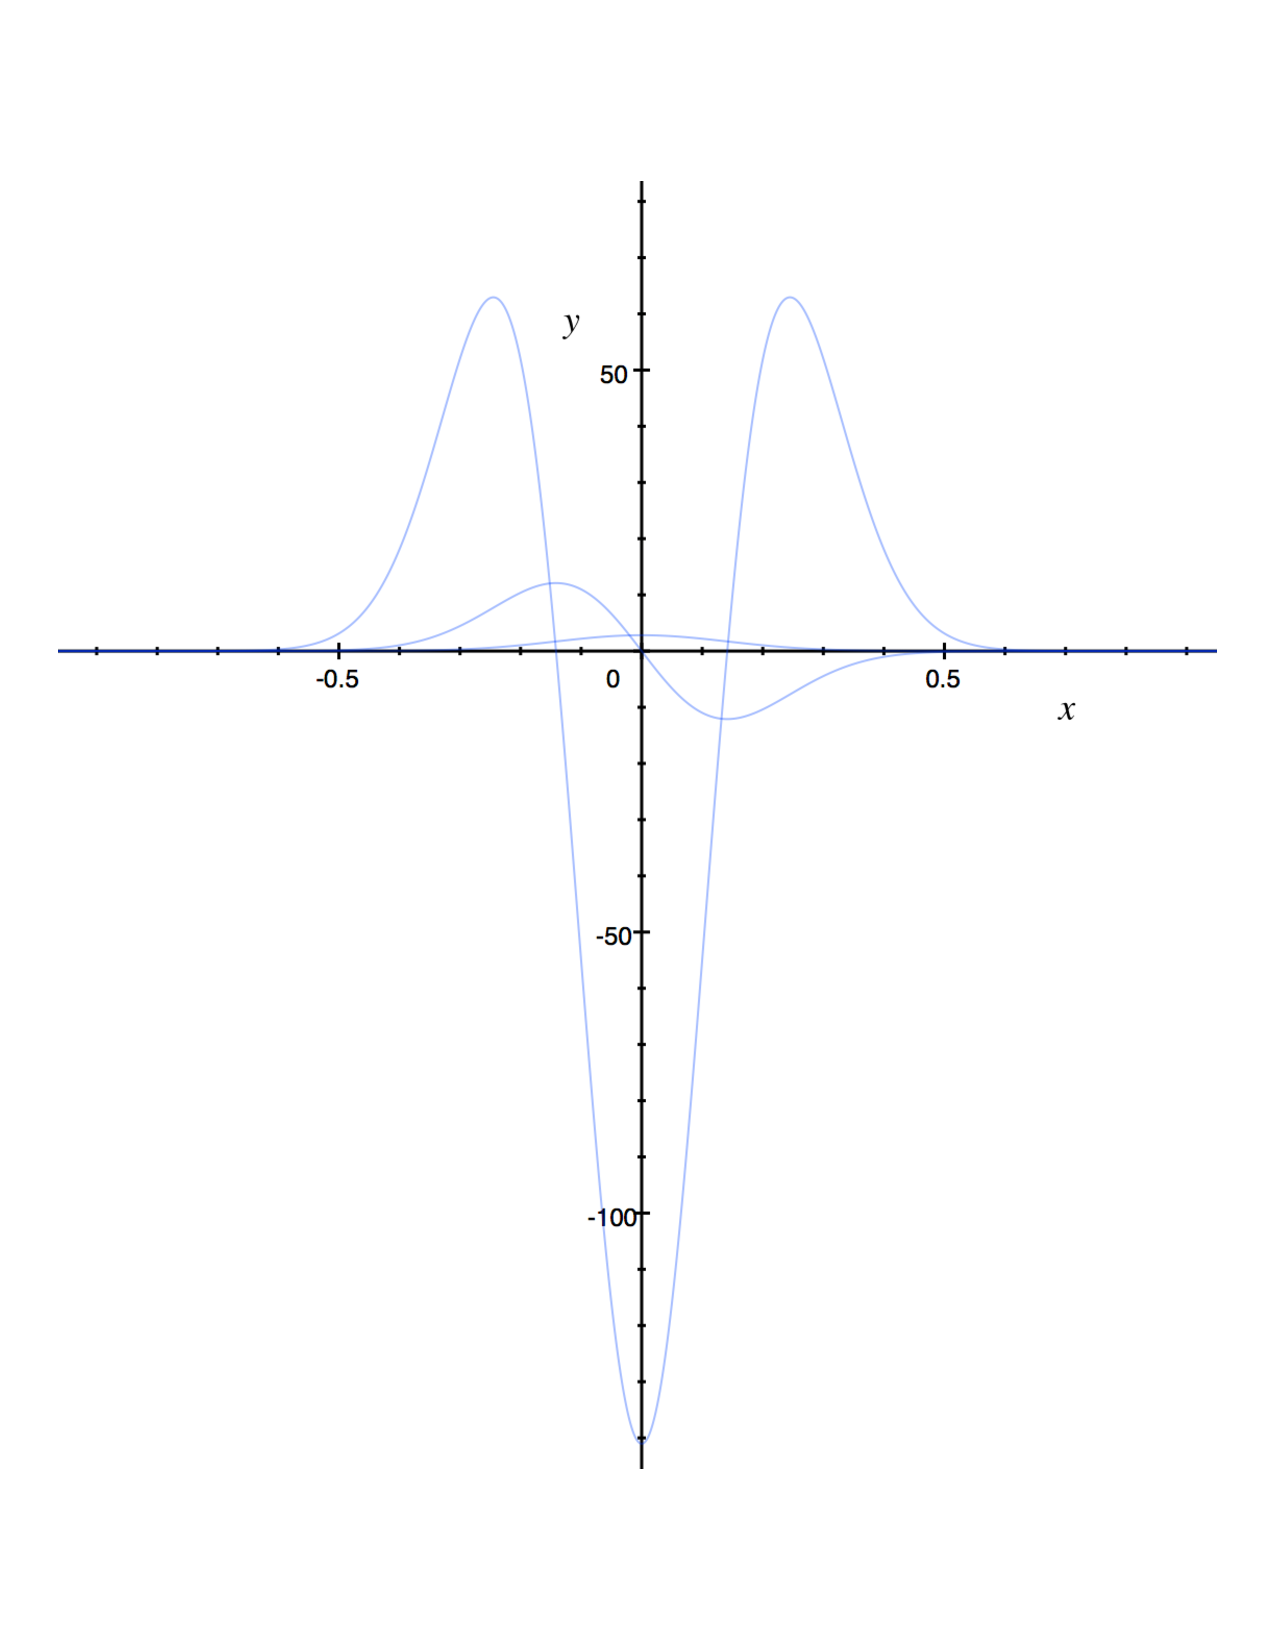
\includegraphics[scale=.25]{ss1.pdf}
\end{center}
\caption{Gaussian representation of $\delta(x)$ and its derivatives ($\Delta=0.2)$}
\end{figure}

\end{document}